\chapter{Signal Generating System}

\section{KAGRA Digital System as Signal Generator}
The Digital Control System used in KAGRA is based on the Advanced LIGO Digital System. In this system, analog control signals can be generated from a Digital-Analog Convertor(DAC) installed in any realtime computer known as a Front-End machine in the tunnel. Between the DAC output and experimental device, a customized analog low-pass filter called an Anti-Image filter has been installed for removing unwanted high frequency signal, the Image, due to digitized output from DAC. 

Inside the Front-End machines, the signal that will be sent to DAC are prepared by realtime software, which is generated from several building blocks, the realtime models, by customized parser and compiler. Each realtime model will be running at specifiable sample rate on a dedicated CPU core. However, currently, all DAC cards installed at KAGRA site are 16bit, 64kHz (65536Hz) ones. Therefore, a mandatary model named Input/Output Processor(IOP) model will always run at 64kHz, communicating with a DAC card and other "slave" models, in which 

(people) 

can put digital filters, signal generators, etc.


\section{Noise Problem of Injection Signal}


\begin{figure}[hbt!]
\centering
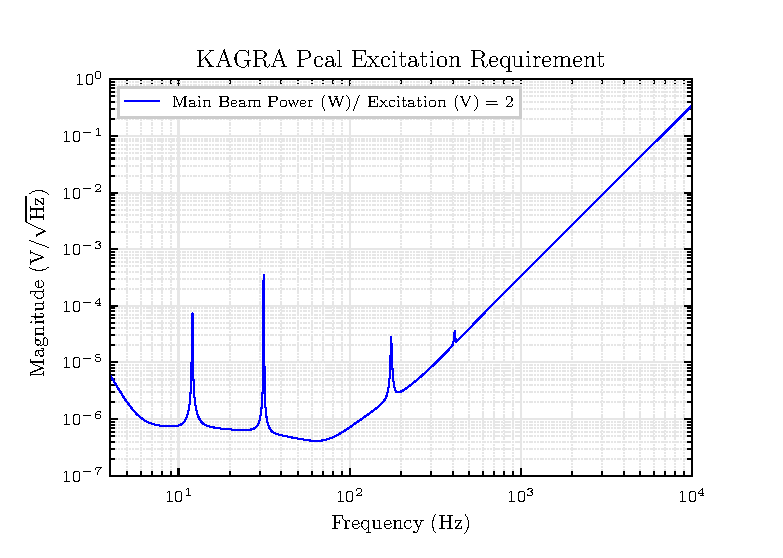
\includegraphics[width=.9\textwidth]{figure/DAC_requirement.eps}
\caption{Injection Channel Noise Requirement}\label{fig:DAC_noise_requirement}
\index{figures}
\end{figure}

\begin{align}
%\label{eq:}
   \Delta L(f) &< \frac{1}{10} \times (\text{KAGRA length sensitivity})\\
   \Delta L(f) =\frac{2 \Delta P(f) \cos(\theta)}{c} \frac{1}{M(2 \pi f)^2} &< \frac{1}{10} \Delta h(f) L
\end{align}




\subsection{Noise Sources from Control Signal}
\subsubsection{Quantization Noise of DAC}


The origin of quantization error is coming from the difference between desired analog output and quantized Digital to Analog Converter(DAC) output value. Roughly speaking, it shows up like white noise that is spread from DC to Nyquist frequency, i.e. $Fs/2$.
The Root Mean Square value of quantization noise has the order of voltage difference corresponding to last digit or Least Significant Bit(LSB). In time domain, we can calculate standard deviation.
\begin{align}
%\label{eq:}
   \sigma_x = \sqrt{\frac{1}{12}} \delta x_{LSB}
\end{align}

For a 16-bit 64kHz DAC with output range between $\pm 10$Volts, 
\begin{align}
%\label{eq:}
    \sigma_x &= \sqrt{\frac{1}{12}} \delta x_{LSB} \\
             &= \sqrt{\frac{1}{12}} \frac{(+10)-(-10) \mathrm{Volts}}{2^{16}} \\
             &= 8.81 \times 10^{-5} \;\mathrm{Volts}
\end{align}

In frequency Domain, the quantization noise is distributed from DC to 32768Hz; therefore, we have ASD
\begin{align}
%\label{eq:}
    ASD &= \sqrt{PSD} \\
        &= \sqrt{ \frac{\sigma_x^2}{32768} } \\
        &= 8.81 \times 10^{-5} \sqrt{\frac{1}{32768}} \\
        &= 4.87 \times 10^{-7} \;\mathrm{Volts}/\sqrt{\mathrm{Hz}} 
\end{align}

\subsubsection{Analog circuits}


\subsubsection{AC Power Line}


